\section{Success criteria}

The project met all its success criteria:
\begin{todolist}[itemsep=0pt,topsep=5pt]
    \item[\done] Implemented the experimental framework (\graffs) to automate experiments of robustness of graph metrics
    \item[\done] Completed statistical analysis and compared results to The Paper
    \item[\done] Extended the idea from The Paper to unscored networks, and deduced empirical observations about graph metrics on interesting unscored datasets
\end{todolist}

\noindent
I also completed one extension:
\begin{todolist}[itemsep=0pt,topsep=5pt]
    \item[\done] Wrap up \graffs and release it as a library under an open-source licence
\end{todolist}

For the evaluation of \graffs, I designed the following 3 experiments:
\begin{description}[itemsep=\zerospace]
    \item[\texttt{reproduce}] focuses on reproducing some results from The Paper, following the setup from The Paper as closely as possible, carried out on the 3 protein interaction networks (\texttt{pvivax}, \texttt{ecoli}, \texttt{yeast})
    \item[\texttt{random-edges}] validates that random edge deletion is a suitable graph generation method, by applying the same pipeline as in \texttt{reproduce} but with random edge deletion
    \item[\texttt{unscored}] applies the random edge deletion method to new, unscored, datasets
\end{description}


\section{Validation against The Paper}

One of the added values of \graffs is the ability to experiment with \textsl{unscored} graphs.
However, in order to validate whether the results produced by \graffs are legit, I first constructed and ran a \texttt{reproduce} experiment trying to reproduce results from The Paper, by linearly thresholding 3 scored protein interaction networks in the same way as The Paper.

\phantomsection
\label{para:how_to_compare_results}
It is important to note that the robustness values from The Paper and \graffs should not be compared directly as there are many details that make the numerical values vary between implementations.
For example, when ranking nodes according to a metric, The Paper resolved ties randomly for each perturbed graph, while my implementation resolves ties arbitrarily but predictably and constantly across all perturbed graphs of a dataset.
The Paper also randomly resolved ties when calculating the overall ranking (\autoref{def:overall_ranking}).
Furthermore, there are other nuances that may cause differences in numerical results, such as $\alpha,k$ coefficients used for $k$-similarity and $\alpha$-relaxed $k$-similarity\footnote{Different values were used in \graffs to generalize the process. See definitions~\ref{def:k_similarity} and~\ref{def:alpha_relaxed_k_similarity}}, definitions of graph metrics in special cases (such as for isolated nodes), and floating-point arithmetic.
Instead of comparing results numerically, the overall trend is to be considered.

The \texttt{reproduce} experiment and the \texttt{thMedHigh} generator (producing 31 graphs at linearly spaced thresholds between 0.60 and 0.90 confidence values) were set up in the following way:
% @formatter:off
\begin{lstlisting}[language=bash]
graffs dataset download-demos
graffs generator create --name thMedHigh --method threshold-linear --params 600,900 -n 31 --seed 7
graffs experiment create --name reproduce --datasets pvivax,ecoli,yeast --generator thMedHigh --metrics Betweenness,Degree,Ego1Edges,Ego2Nodes,LocalClustering,PageRank,Redundancy --robustnessMeasures RankIdentifiability,RankInstability,RankContinuity
graffs experiment run --name reproduce
\end{lstlisting}
% @formatter:on

As for the set of metrics, I evaluated all that were also evaluated in The Paper, apart from Closeness and Harmonic centrality (Definitions~\ref{eqn:closeness_centrality} and~\ref{eqn:harmonic_centrality}).
These two depend on the all pair shortest paths algorithm with time complexity $O({\left\lvert V \right\rvert}^3)$ that would take unreasonable amount of time to compute on large graphs.

\begin{figure}
    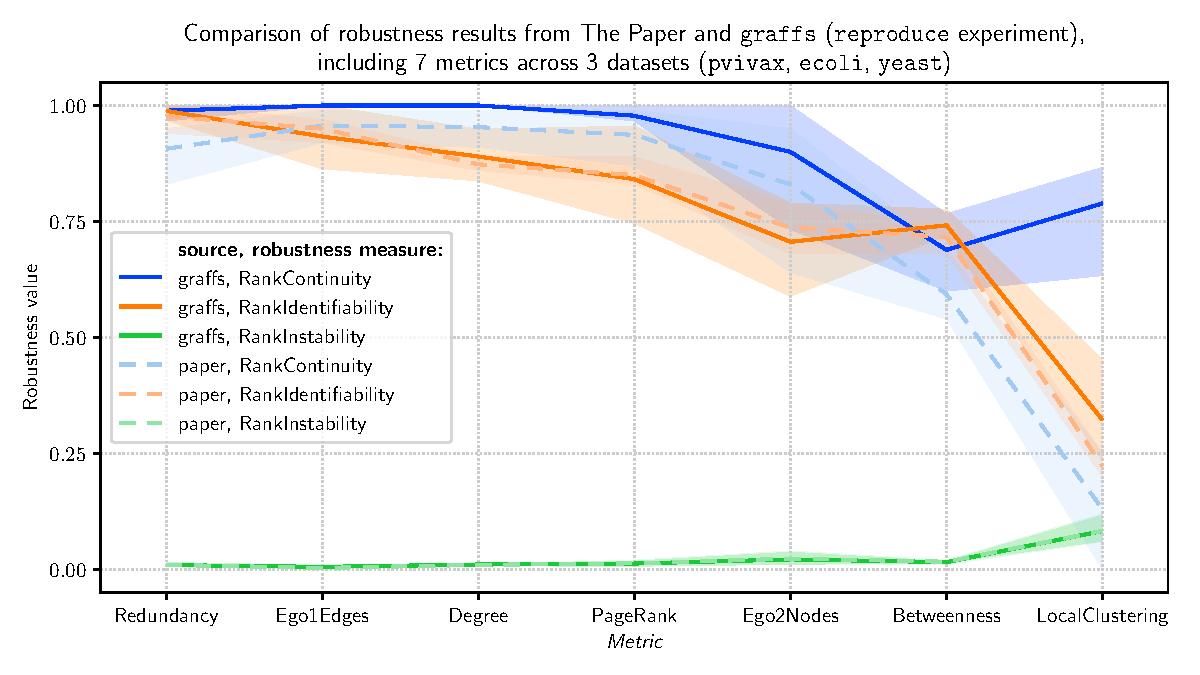
\includegraphics[width=\linewidth]{plot_reproduction.pdf}
    \caption{Comparison of results from The Paper and \graffs.
    Each color corresponds to one robustness measure, with thin lines inside each band showing robustness of individual datasets, and the thick line showing the average robustness across the 3 datasets.
    Solid and dashed bands correspond to results obtained by \graffs and The Paper, respectively.}
    \label{fig:plot_reproduction}
    \footnotesize
    \begin{flushleft}
        Note that high values of RankContinuity and RankIdentifiability mean high \textsl{robustness}, whereas high values of RankInstability mean low \textsl{robustness}.
        Metrics are sorted from left to right by their decreasing combined robustness.
    \end{flushleft}
\end{figure}


Averaging the robustness values across the 3 protein datasets with similar structure, \autoref{fig:plot_reproduction} demonstrates that \graffs is successful in identifying similar robustness properties of metrics as in The Paper.
The Paper identifies metrics \texttt{Ego1Edges}, \texttt{Redundancy}, \texttt{Degree}, and \texttt{PageRank} as very stable (i.e. robust).
Those have reported RankContinuity and RankIdentifiability values above $0.75$ on almost all evaluations on the 3 datasets, and RankInstability below $\sim 0.1$.
\graffs equally reports these metrics as relatively stable.

On the other hand, \texttt{Betweenness} and \texttt{LocalClustering} are considered unstable by The Paper (RankContinuity and RankIdentifiability significantly dropped while RankInstability increased), and the results from \graffs copy the behaviour.
Although the RankContinuity values of \texttt{LocalClustering} are not as low as reported by The Paper, one can definitely conclude that these two metrics are equally identified as less robust by \graffs.

For further thought, we can also consider variance of robustness measures, concluding, for example, that \texttt{Redundancy} (a stable metric) has small variance in RankIdentifiability across the 3 datasets as reported by \graffs, whereas the RankContinuity and RankIdentifiability of the \texttt{Ego2Nodes} metric led to more diverse values.

\subsection{Rank similarity}

Another way to validate intermediate results is to consider $k$-similarity of perturbed graphs between two consecutive thresholds, and $\alpha$-relaxed $k$-similarity between graphs at individual thresholds and overall ranks.
For each dataset \texttt{pvivax}, \texttt{ecoli}, \texttt{yeast}, I generated $85$ graphs thresholded at values between $0.15$ and $0.99$, and calculated the needed metric values for each graph.
Then I compare the results for 3 chosen metrics on the protein network datasets with the results of The Paper.

\afterpage{%
    \begin{savenotes}%
        \begin{figure}[H]
            \begin{enumerate}
                \item[(a)] 
\includegraphics[scale=0.99]{plot_rank_similarity_papertop.pdf}\\
                \vspace*{-0.2cm}%
                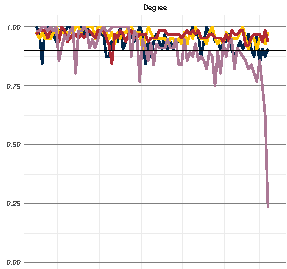
\includegraphics[scale=0.99]{plot_rank_similarity_paper_degree.pdf}\hspace*{0.1mm}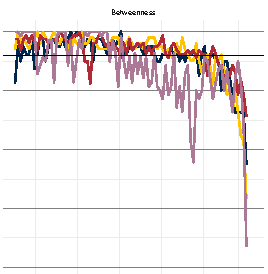
\includegraphics[scale=0.99]{plot_rank_similarity_paper_betweenness.pdf}\hspace*{-0.4mm}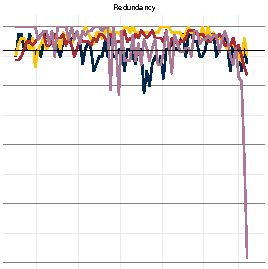
\includegraphics[scale=0.99]{plot_rank_similarity_paper_redundancy.pdf}\\
                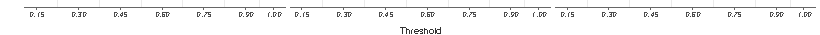
\includegraphics[scale=0.99]{plot_rank_similarity_paperbottom.pdf}
                \vspace*{-0.7cm}
                \item[(b)] \hspace*{-0.25cm}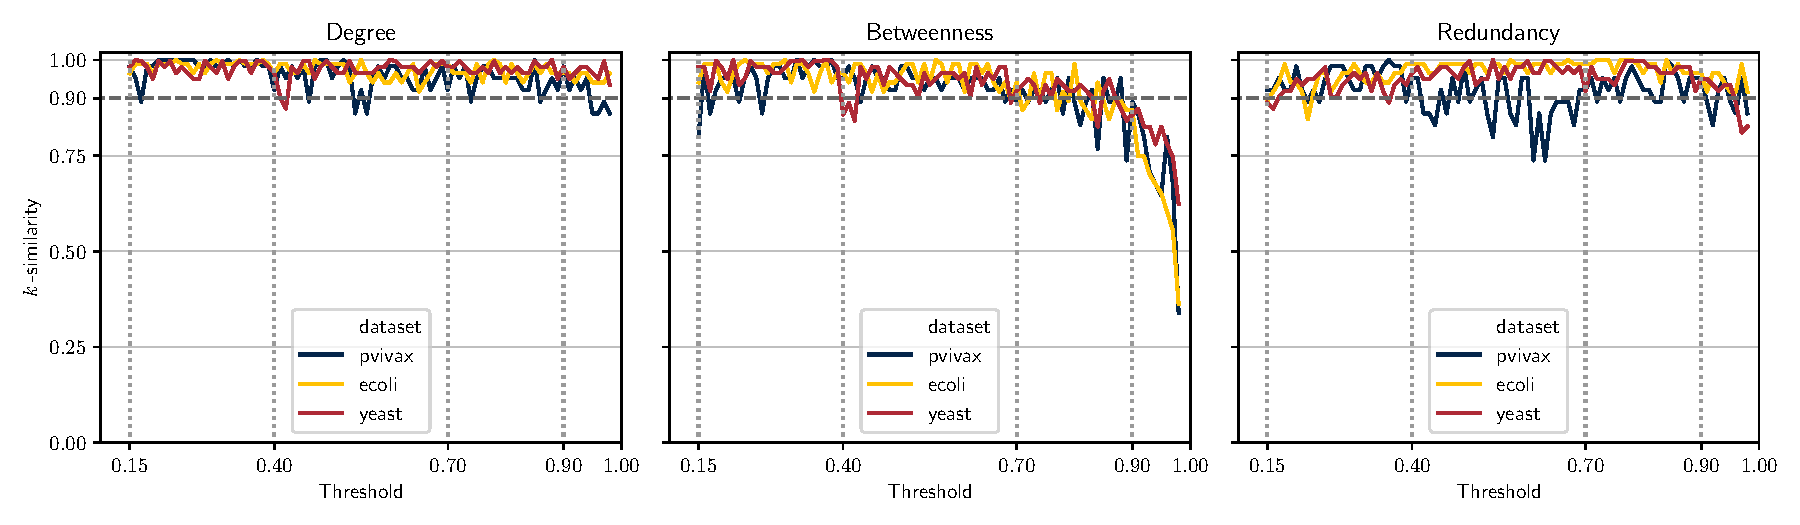
\includegraphics[align=t,width=0.96\linewidth]{plot_rank_similarity_graffs.pdf}
            \end{enumerate}
            \caption{$k$-similarity plots between ranks of graphs derived from protein networks\cref{foot:hpred} at consecutive thresholds, taking results from The Paper~(a) and \graffs~(b).\cref{foot:similarity_coefficients}}
            \label{fig:plot_rank_similarity}
            \vspace*{-0.4cm}
%\footnotetext{\label{foot:similarity_coefficients}Chosen according to \url{https://github.com/lbozhilova/measuring_rank_robustness/blob/master/figure_generation.R#L28}}
            \begin{enumerate}
                \item[(a)] 
\includegraphics[scale=0.99]{plot_relaxed_similarity_papertop.pdf}\\
                \vspace*{-0.2cm}%
                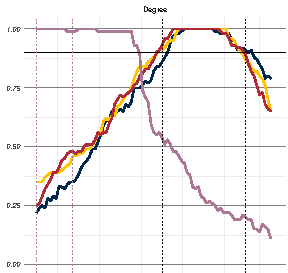
\includegraphics[scale=0.99,trim={0 0.8mm 0 0},clip]{plot_relaxed_similarity_paper_degree.pdf}\hspace*{0.2mm}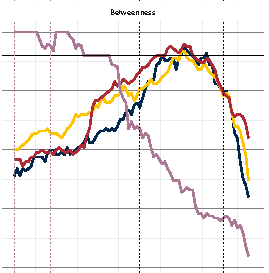
\includegraphics[scale=0.99,trim={0 0.3mm 0 0},clip]{plot_relaxed_similarity_paper_betweenness.pdf}\hspace*{-0.45mm}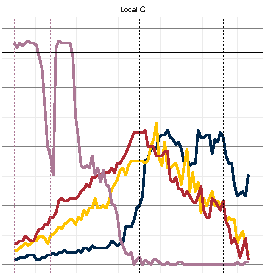
\includegraphics[scale=0.99,trim={0 0.8mm 0 0},clip]{plot_relaxed_similarity_paper_localc.pdf}\\
                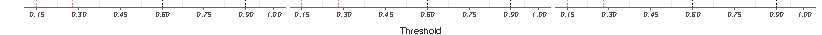
\includegraphics[scale=0.99]{plot_relaxed_similarity_paperbottom.pdf}
                \vspace*{-0.7cm}
                \item[(b)] \hspace*{-0.25cm}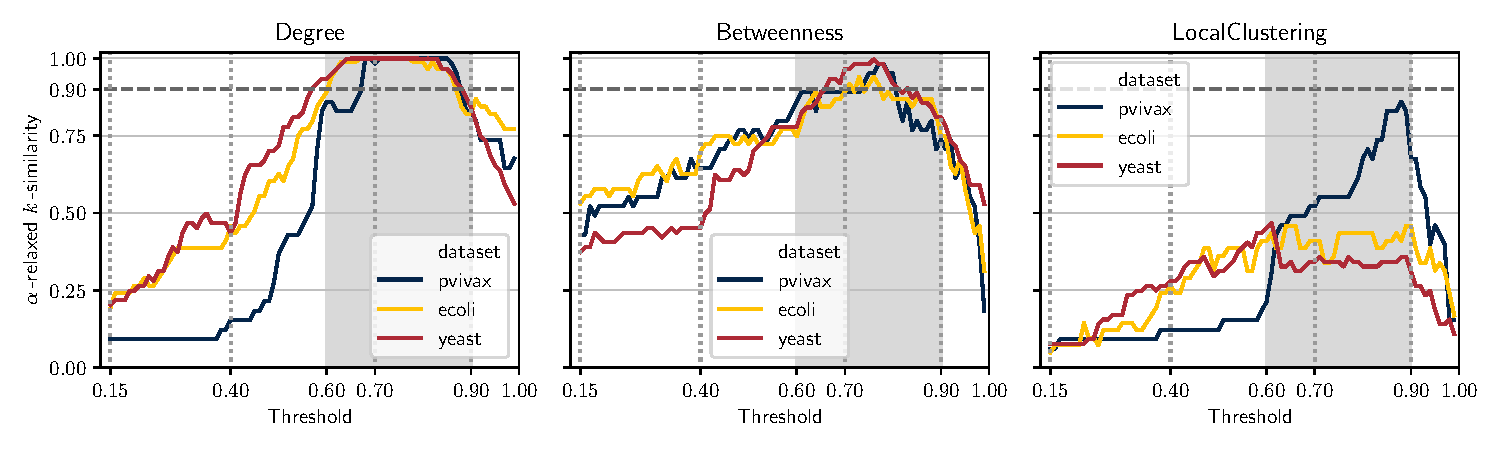
\includegraphics[align=t,width=0.96\linewidth]{plot_relaxed_similarity_graffs.pdf}
            \end{enumerate}
            \caption{$\alpha$-relaxed $k$-similarity plots between overall rank and ranks at individual thresholds, taking results from The Paper~(a) and \graffs~(b) on protein networks\protect\footnote{\label{foot:hpred}The HPRED dataset is not used in this dissertation and so is irrelevant}.
            The overall rank for each of 3 metrics was calculated within the ``wide medium-high confidence region'' $\left[ 0.6, 0.9 \right]$.\protect\footnote{\label{foot:similarity_coefficients}Coefficients were set to $k=0.01, \alpha=1.5$, as in the source code of experiments done in The Paper: \url{https://github.com/lbozhilova/measuring_rank_robustness}}}
            \label{fig:plot_relaxed_similarity}
        \end{figure}%
        \vspace{-1cm}
    \end{savenotes}
%\footnotetext{Chosen according to \url{https://github.com/lbozhilova/measuring_rank_robustness/blob/master/robustness_analysis_aux.R#L108}}
    \clearpage}


\autoref{fig:plot_rank_similarity} shows $k$-similarity of each pair of graphs at consecutive thresholds, along with plots of the same data from The Paper.
The $k$-similarity values are used for calculating \texttt{RankContinuity}, which is equal to the proportion of such pairs of consecutive graphs whose $k$-similarity is above the $0.9$ threshold (\autoref{def:rank_continuity}).

\autoref{fig:plot_relaxed_similarity} shows $\alpha$-relaxed $k$-similarity between overall ranking and rankings of graphs at individual thresholds.
The $\alpha$-relaxed $k$-similarity is used for calculating \texttt{RankIdentifiability}, which is equal to the minimum similarity value within the $\left[ 0.6, 0.9 \right]$ confidence interval (\autoref{def:rank_identifiability}).

The visual plots of the three chosen metrics in each case demonstrate that \graffs's similarity values match those of The Paper closely, in both $k$-similarity and $\alpha$-relaxed $k$-similarity.


\section{Validation of random edge deletion}

Randomly deleting a small subset of edges allows us to evaluate robustness of metrics on unscored graphs.
The purpose of the \texttt{random-edges} experiment is to justify reliability and accuracy of this approach, comparing robustness results of the same metrics, on the same datasets, but with a different graph-generating method.

\begin{wrapfigure}{R}{0.5\textwidth}
    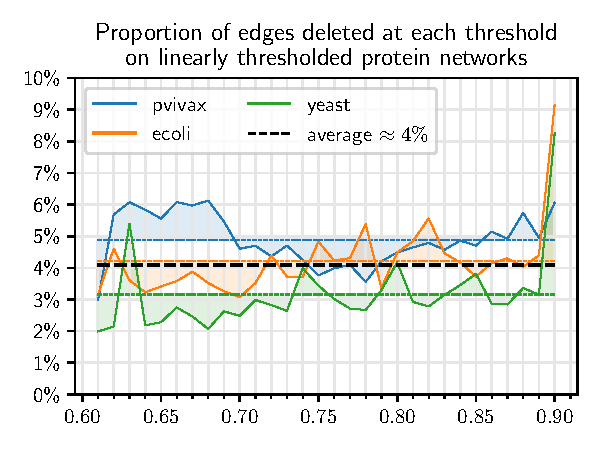
\includegraphics[width=\linewidth]{plot_edge_deletion_per_step.pdf}
    \vspace*{-0.5cm}
    \caption{Proportion of deleted edges in 3 protein network (around $4\%$ at each threshold)}
    \label{fig:plot_edge_deletion_per_step}
\end{wrapfigure}


To start, I needed to choose the $\delta$ parameter for $\mathlarger{^{ER} \mathlarger{\xi}}_\delta$, the edge-removing graph generator (see \autoref{eq:edge_removing_generator}).
Considering the distribution of confidence scores (\autoref{fig:histogram_edges}), I derived its right-to-left cumulative distribution (\autoref{fig:plot_cumulative_confidence_scores}) and differentiated to get a decrease rate at each threshold, as seen in \autoref{fig:plot_edge_deletion_per_step}.
As calculated, the relative amount of edges deleted when increasing the threshold in $0.01$ increments (as practiced in The Paper), is $4\%$ in average.
Thus, I set $\delta=0.04$ (proportion of edges to delete) in the random edge deletion algorithm.

To make this graph generator work on unscored graphs comparably to scored graphs as in the previous experiment, I also set the \textsl{initial threshold} of each scored graph to the confidence of $0.6$.

The experiment was set up using the following commands:
% @formatter:off
\begin{lstlisting}[language=bash]
graffs dataset download-demos
graffs generator create --name random04 --method removing-edges --params 0.04,600 -n 31 --seed 7
graffs experiment create --name random-edges --datasets pvivax,ecoli,yeast --generator random04 --metrics Betweenness,Degree,Ego1Edges,Ego2Nodes,LocalClustering,PageRank,Redundancy --robustnessMeasures RankIdentifiability,RankInstability,RankContinuity
graffs experiment run --name random-edges
\end{lstlisting}
% @formatter:on

\begin{figure}
    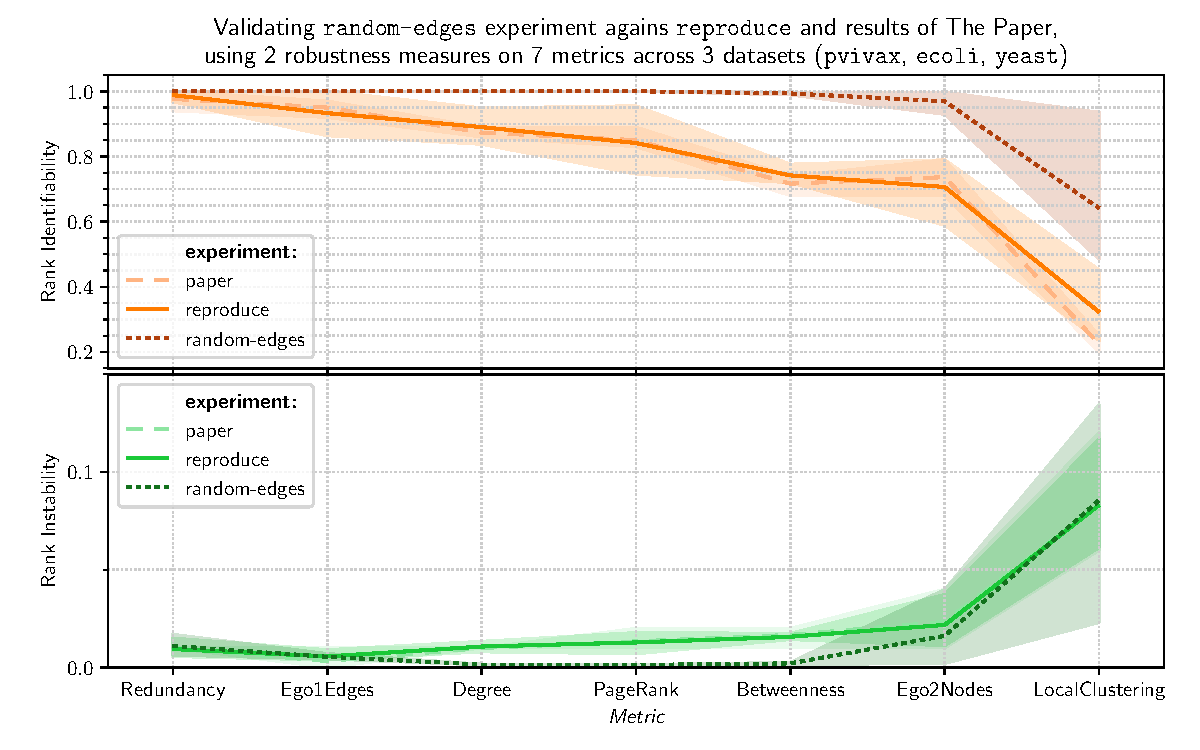
\includegraphics[width=\linewidth]{plot_random_edges.pdf}
    \caption{Validation of the \texttt{random-edges} experiment against \texttt{reproduce} and results of The Paper, using RankIdentifiability and RankInstability (displayed separately) on 7 metrics across 3 datasets.
    Thin lines inside each color band band show robustness of individual datasets, and the thick line shows the average robustness across the 3 datasets.
    Each line style (solid, long dashes, short dashes) corresponds to results obtained from different experiment or source.}
    \label{fig:plot_random_edges}
    \footnotesize
    \begin{flushleft}
        High values of RankIdentifiability mean high \textsl{robustness}, whereas high values of RankInstability mean low \textsl{robustness}.
        Metrics are sorted from left to right by their decreasing combined robustness.
    \end{flushleft}
\end{figure}


Results are shown in \autoref{fig:plot_random_edges}.
We can see that all 3 robustness measures follow the expected behaviour for the two less-stable metrics \texttt{Ego2Nodes} and \texttt{LocalClustering}.
However, RankContinuity is not able to mark \texttt{Betweenness} as less stable, and even shows zero variance for \texttt{Betweenness}.

RankContinuity is different from the other two metrics, in that it explicitly uses perturbed graphs in a sequence, considering differences between pairs of consecutive graphs.
The different behaviour of RankContinuity can perhaps be explained by that the \texttt{random-edges} graph generator removes edges uniformly at each step, whereas \texttt{threshold-linear} removes edges according to a non-uniform distribution of edge scores.\footnote{In protein networks that were used as a baseline for this experiment, edges likely do not have all of their scores independent of each other, but rather dependent on local proximity of each edge.}

Note again, that the results of the experiments are not expected to match numerically, due to numerous changes and generalisations in \graffs as opposed to The Paper, only to yield similar behaviour (as explained in \autoref{para:how_to_compare_results}).
Overall, the results show that randomly removing edges is a suitable substitute for linear thresholding.


\section{Extending to unscored datasets}

Having validated that randomly removing edges is a reasonable method for generating small perturbations in unscored graphs, we can now proceed to evaluating robustness of multiple metrics on multiple interesting datasets.
For this, I used the 5 unscored datasets (described in~\autoref{sec:unscored_datasets}): \texttt{airports}, \texttt{citation}, \texttt{collab}, \texttt{facebook}, \texttt{internet}.

The experiment is set up as follows:
% @formatter:off
\begin{lstlisting}[language=bash]
graffs dataset download-demos
graffs experiment create --name unscored --generator random04 \
    --datasets airports,citation,collab,facebook,internet \
    --metrics Betweenness,Degree,Ego1Edges,Ego2Nodes,LocalClustering,PageRank,Redundancy \
    --robustnessMeasures RankIdentifiability,RankInstability,RankContinuity
graffs experiment run --name unscored
\end{lstlisting}
% @formatter:on

\begin{figure}
    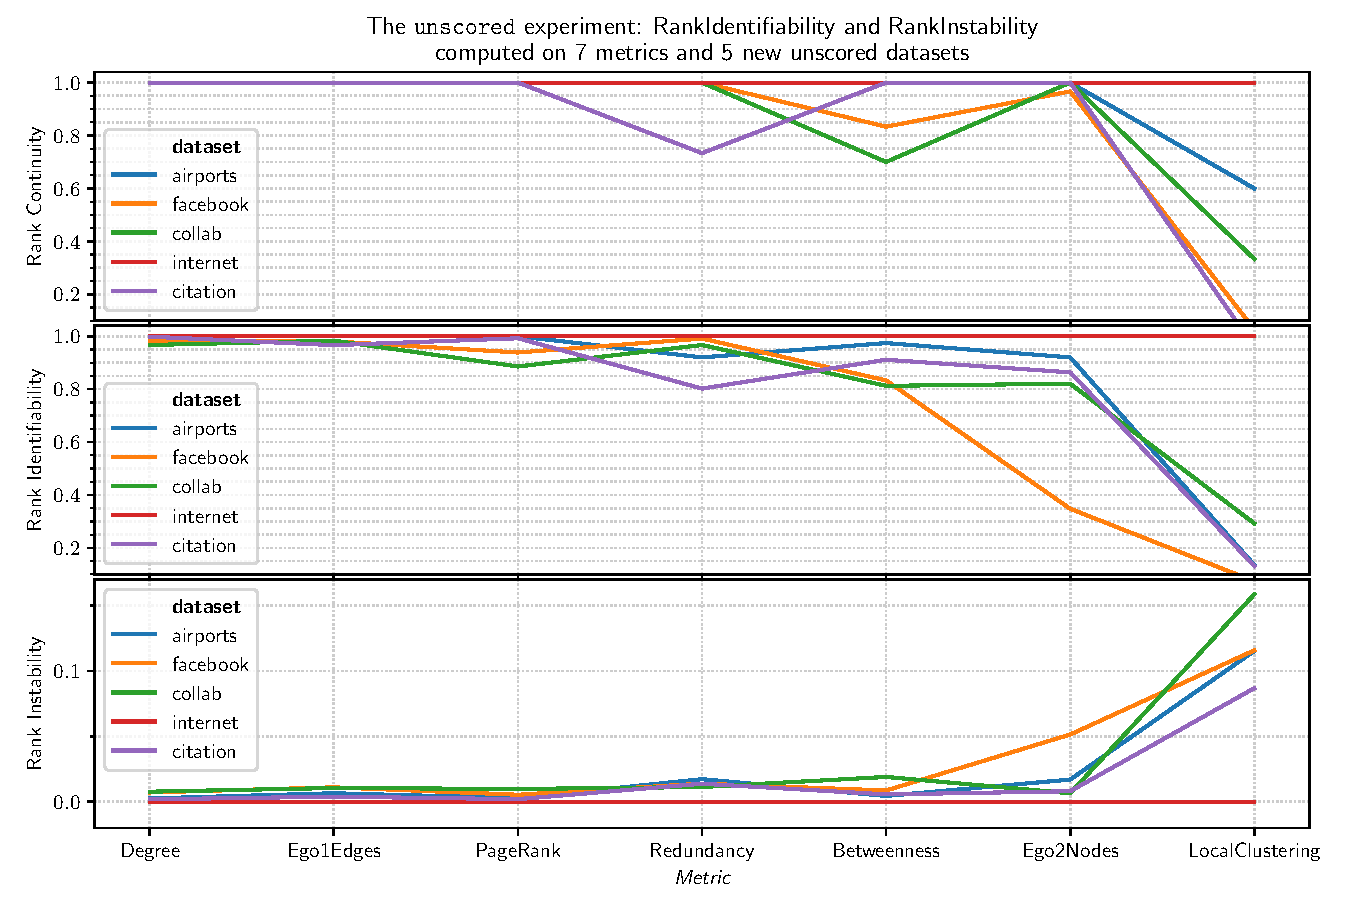
\includegraphics[width=\linewidth]{plot_unscored.pdf}
    \vspace*{-0.6cm}
    \caption{Evaluating RankContinuity, RankIdentifiability and RankInstability on 5 new unscored datasets, generating graphs by randomly deleting $4\%$ of edges.}
    \label{fig:plot_unscored}
    \footnotesize\justify\vspace{-0.4\baselineskip}
    High values of RankContinuity and RankIdentifiability mean high robustness, whereas high values of RankInstability mean low robustness.
    Metrics are sorted from left to right by their decreasing combined robustness.
\end{figure}


\autoref{fig:plot_unscored} shows 3 robustness measures evaluated on the 7 metrics using 5 unscored datasets.
Overall, the tendency of robustness measures identify the key results from previous experiments: metrics \texttt{Degree}, \texttt{Ego1Edges}, and \texttt{PageRank} are mostly stable on all datasets.
The \texttt{facebook} dataset has relatively lower RankIdentifiability of \texttt{Ego2Nodes} metric, and most of the datasets apart from \texttt{internet} have lower stability of the \texttt{LocalClustering} and \texttt{Ego2Nodes} metrics.

\Cref{tab:robustness-continuity,tab:robustness-identifiability,tab:robustness-instability}, included in \cref{ch:appendix_results}, show the numerical results of all the results presented here, and in the previous \texttt{random-edges} experiment.

There are a number of interesting observations about the new datasets.

\begin{enumerate}
    \item The \texttt{LocalClustering} metrics is unstable in general, but yields the same stability as other stable metrics for the \texttt{internet} dataset, thus, there must be something interestingly \textsl{different} with the hierarchy of autonomous systems of the Internet.
    Ideally, we would be able to quantify this using some (possibly other) graph metrics.

    \item RankContinuity does not report \texttt{Ego2Nodes} as significantly less stable for any of the datasets, unlike other robustness measures.
    This can, perhaps, be explained by the fact that the nodes with highest ranks induced by \texttt{Ego2Nodes} have the ego-2 network too big for the uniform edge deletion to make any significant change in their ranks ranks.
    \item The \texttt{facebook} belongs to the less stable datasets for most of the metrics.
    This might be explained by the fact that in a social network, there are perhaps many similarities in the structural patterns (usual degrees of nodes, density of connected cliques or communities, etc.), as opposed to other graphs with highher diversity, and so smaller differences in absolute metric values are needed to trigger changes in ranks.

    However, the possible explanations are not based on any statistical analysis, and are open to yet another research.
\end{enumerate}

An interesting thought for the future is finding a correlation between robustness of metrics on graphs and their structure, or the values of some other graph metrics.
Ideally, one would be able to reason about robustness of a graph metrics on a graph purely based on the values of some other metrics of the graph (which themselves may be stable or unstable, too), without the need to simulate graph petrurbations.
My work does not include, and was not expected to include this kind of analysis due to the limits of its extent -- having enough of data finding correlations between metrics values and robustness of metrics would require an order of magnitude more evaluations.
However, the \graffs tool I developed is powerful enough to be able to facilitate this kind of analysis, given more time, computing power and resources for further investigation, and it can easily be extended to do so.


\section{Performance}

\begin{table}
    \centering
    \caption{CPU Computation time of the 3 experiments evaluated by \graffs, run on the \texttt{rio} computing cluster (see \autoref{sec:computing_cluster}).
        \textsl{Total CPU time} is the sum of all times of individual CPU cores spent on evaluating the experiment, and \textsl{Avg CPU time per graph} is that divided by $(\text{number of datasets}) \times (\text{number of graphs generated from each dataset})$.}
    \label{tab:perf_experiments_table}
    % @formatter:off
    \begin{tabular}{|l|r|r|}
    \toprule
                Experiment &             Total CPU time & Avg CPU time per graph \\
    \midrule
        \texttt{reproduce} &          13 hours, 17 mins &                 9 mins \\
     \texttt{random-edges} &          22 hours, 36 mins &                15 mins \\
         \texttt{unscored} &  9 days, 12 hours, 57 mins &        1 hour, 29 mins \\
    \bottomrule
    \end{tabular}
    % @formatter:on
\end{table}


\begin{wrapfigure}[13]{r}{0.45\textwidth}
    \vspace{-0.6cm}
    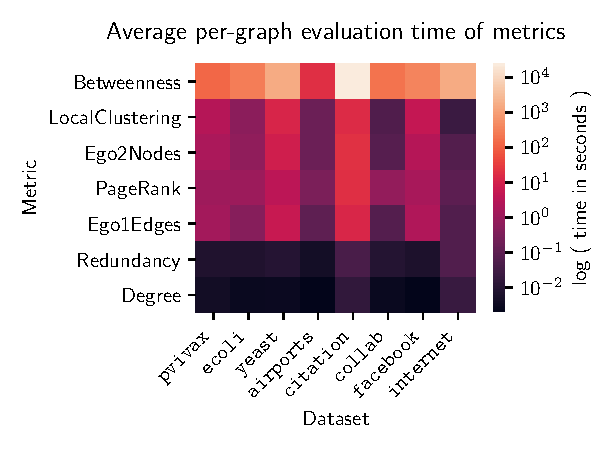
\includegraphics[width=\linewidth]{perf_timings_matrix.pdf}
    \vspace{-0.8cm}
    \caption{Per-graph evaluation time of metrics, averaged over graphs generated from various datasets}
    \label{fig:perf_timings_matrix}
\end{wrapfigure}


\Cref{tab:perf_experiments_table} compares the time it took to evaluate the experiments: \texttt{reproduce}, \texttt{random-edges}, \texttt{unscored}; and the time spent on evaluating each graph.
The performance of the experiments was measured on the \texttt{rio} computing cluster (see \autoref{sec:computing_cluster}).
The table measures total CPU times, therefore assuming that $n$ cores run in parallel and the machine executes no other processes in the meantime, the real (wall-clock) duration of each experiment is then $n$-times shorter.
This value is useful to compare the \textsl{absolute computational complexity} of each experiment, as it does not depend on the number of cores, and neither the fraction of the program that is perfectly parallelised.

\Cref{fig:perf_timings_matrix} compares the logarithm of the time it took to evaluate each metric on a single graph, in average, taking measurements from the 3 experiments \texttt{reproduce}, \texttt{random-edges}, and \texttt{unscored}.
We can see that the betweenness centrality is most computation heavy, with the computation taking more than an hour in average for a single graph generated from the \texttt{citation} dataset.
This is presumably because the \texttt{citation} dataset is much bigger in the number of edges compared to the other used datasets.


%\section{Releasing \graffs}

%\todo{Make graffs citable}
%https://guides.github.com/activities/citable-code/
